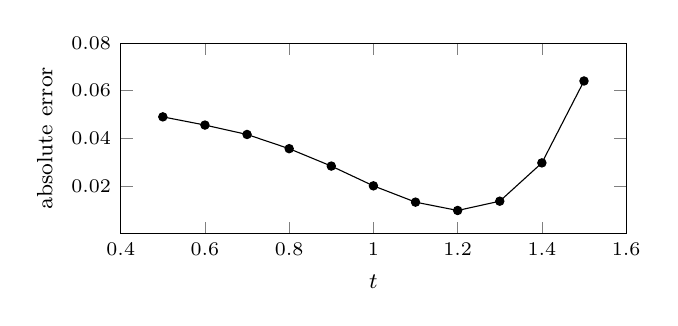
\begin{tikzpicture}
\begin{axis}[
    xlabel=\footnotesize{$t$},
    ylabel=\footnotesize{absolute error},
    xmin = 0.4, xmax = 1.6,
    xtick = {0.4,0.6,0.8,1.0,1.2,1.4,1.6},
    ymin = 0, ymax =0.08,
    ytick = {0.02,0.04,0.06,0.08},
    width=8cm,height=4cm,
    font = \scriptsize,
    scaled y ticks = false,
    yticklabel style={
            /pgf/number format/fixed,
        },
]
% \addplot[color=red]{exp(x)};
\addplot[mark=*,black,mark size=1.5pt] plot coordinates {
    (1.5,0.0641)
    (1.4,0.02969)
    (1.3,0.0136)
    (1.2,0.0097)
    (1.1,0.0132)    
    (1,0.02005)   
    (0.9,0.02835)   
    (0.8,0.03566)
    (0.7,0.04163)   
    (0.6,0.04558)   
    (0.5,0.04903)           
};
\end{axis}
\end{tikzpicture}
